
\section{mbiclique.rb - Enumerate Maximal Bipartite Cliques\label{sect:mbiclique}}

This command enumerates maximal bipartite clique from bipartite graph. The \verb|lcm| command \cite{UnoWeb} is used in mbiclique.rb. 
It is an bipartite graph represented as $G=(V_1 \cup V_2,E)$, with 2 nodes set  $V_1,V_2$ and edge set connecting to the subsets $E\subset V_1\times V_2$, any node in subgraph $V_1,V_2$  is connected with an edge in $G$ is a directional subgraph.

%$V$の部分集合$V'$に対して$V'$によって誘導される部分グラフ$G'=(V',E(V'))(E'=\{(u,v) \in E|u,v \in V'\}$が完全グラフとなっている$G$の誘導部分グラフをクリークとい>う。
In addition, if the bipartite clique is independent and does not exist in other bipartite cliques, it is referred to as maximal bipartite clique (Figure \ref{fig:biclique}).

\begin{figure}[htbp]
\begin{center}
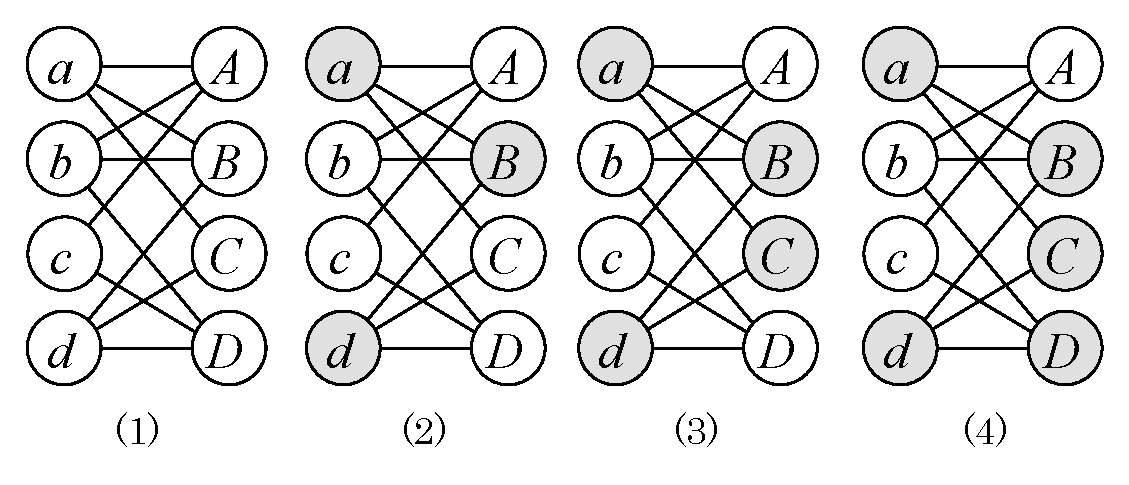
\includegraphics[scale=0.5]{./biclique.eps}
\caption{The shaded nodes in the subgraph from bipartite graph (1) is known as bipartite clique (2),  (3) is a subset of bipartite clique, therefore it is not maximal bipartite clique.  On the other hand, since (3) is not a subset of other bipartite clique, and thus it is maximal. In (4), there is no edge between $a,D$, thus it is not a bipartite clique.    \label{fig:biclique}}
\end{center}
\end{figure} 

Let's consider some real world application for maximal bipartite clique. 
For example, the set of panel data on consumer food purchasing consists of product information and shop information, a bipartite graph can be constructed by connecting product-shop information with an edge for purchases above a certain threshold. 
By enumerating maximal bipartite clique, it is possible to group products and shops with strong relationships. 

This is regarded as particle and noun phrases in text mining. In application, bipartite graph is constructed of particle-noun phrases connected by an edge.  
The basic concept is to enumerate maximal bipartite clique, case frame (particle-noun phrase) with strong relationships will be grouped together. 

When applying this concept in auction data, when the bidder and artifact is taken into consideration, bipartite graph can be constructed by adding edges between bidder-artifact whenever there is a bid.  

The input data for bipartite graph used for the command is shown in \ref{tbl:bicl_input}, edge data is represented in node pairs in CSV format (corresponds to Figure \ref{fig:biclique} (1)). Each item represents a section. 

In Table \ref{tbl:bicl_input}, in column \verb|node1|, the lower-case letters represent the elements, in column  \verb|node2|, the upper-case letters represent elements in other parts.   

The graph is treated as undirected graph and may have more than one island.  

The output of maximal bipartite cliques enumerated from the bipartite graph is shown in Table \ref{tbl:bicl_output}. 

One row corresponds to maximal bipartite clique, the elements that created each section is saved in column \verb|node1,node2| in vector format. 
The size (number of nodes) of each section is saved in \verb|size1,size2|. 

Figure \ref{fig:biclique}(3) corresponds to maximal bipartite clique in row 5 ($V_1=\{a,d\},V_2=\{B,C\}$). 

\vspace{1em}

\begin{table}[htbp]
\begin{center}
\begin{tabular}{cc}

\begin{minipage}{0.3\hsize}
\begin{center}
\caption{Input Data(Edge Data)\label{tbl:bicl_input}}
{\small
\begin{tabular}{cc}
\hline
node1&node2 \\
\hline
a&A \\
a&B \\
a&C \\
b&A \\
b&B \\
b&D \\
c&A \\
c&D \\
d&B \\
d&C \\
d&D \\
\hline
\end{tabular} 
}
\end{center}
\end{minipage}

\begin{minipage}{0.3\hsize}
\begin{center}
\caption{Output Results\label{tbl:bicl_output}}
{\small
\begin{tabular}{llcc}
\hline
node1&node2&size1&size2 \\
\hline
a&A B C&1&3 \\
a b&A B&2&2 \\
a b c&A&3&1 \\
a b d&B&3&1 \\
a d&B C&2&2 \\
b&A B D&1&3 \\
b c&A D&2&2 \\
b c d&D&3&1 \\
b d&B D&2&2 \\
d&B C D&1&3 \\
\hline
\end{tabular} 
}
\end{center}
\end{minipage}

\end{tabular} 
\end{center}
\end{table} 

\subsection{Format}
\begin{verbatim}
Format) mbiclique.rb i= f= [o=] [l=] [u=] [T=] [-debug] [--help]

  Specify File Name
  i= :  Edge data file 
  f= :  Column names of the 2 nodes in edge data
  o= : Output file
  l= : Minimal number of nodes constructing the maximal bipartite cliques.
     : Maximal bipartite cliques smaller than the the value specified here will not be enumerated. 
     : If the values are separated by comma, the size of each can be limited. 
     : Order of values separated by comma corresponds to the order of items specified at f=. 
     : When the limit is not defined, null character can be used  as in "l=2," and "l=,2".
     : Null character in the end can be omitted ("l=2," and "l=2" has the same meaning).
  u= : Maximal number of nodes constructing maximal bipartite clique 
     : Specification details is the same as I= parameter. 

  Others
  T= : Working directory (default:/tmp)
  --help : Help information 
\end{verbatim}

\subsection{Notes}
The output format of bipartite clique in this command is in vector format (a CSV column with character string delimited by space ), sometimes the length of one field can become very long.  
Thus, an error may return if the length of one row of CSV data exceeds the maximum limit when processing the data within MCMD command. 
In this case, the error can be avoided by setting constraints for the bipartite clique at  \verb|l=| and \verb|u=|. 


\subsection{Examples}
\subsubsection*{例1: 基本例}

前節の解説で用いてる例。


\begin{Verbatim}[baselinestretch=0.7,frame=single]
$ more dat.csv
node1,node2
a,A
a,B
a,C
b,A
b,B
b,D
c,A
c,D
d,B
d,C
d,D
$ mbiclique.rb ei=dat.csv ef=node1,node2 o=result1.csv
#MSG# converting paired form into transaction form ...
#MSG# lcm_20140215 CIf /tmp/__MTEMP_95686_70245679198320_0 1 /tmp/__MTEMP_95686_7024567919
8320_3
trsact: /tmp/__MTEMP_95686_70245679198320_0 ,#transactions 4 ,#items 4 ,size 11 extracted 
database: #transactions 4 ,#items 4 ,size 11
 output to: /tmp/__MTEMP_95686_70245679198320_3
separated at 0
iters=11
11
1
3
4
3
#END# /usr/bin/mbiclique.rb ei=dat.csv ef=node1,node2 o=result1.csv
$ more result1.csv
node1,node2,size1,size2
a,A B C,1,3
a b,A B,2,2
a b c,A,3,1
a b d,B,3,1
a d,B C,2,2
b,A B D,1,3
b c,A D,2,2
b c d,D,3,1
b d,B D,2,2
d,B C D,1,3
\end{Verbatim}
\subsubsection*{例2: サイズを制限する例}

項目\verb|node1,node2|共にサイズが2の極大二部クリークを列挙する。


\begin{Verbatim}[baselinestretch=0.7,frame=single]
$ mbiclique.rb ei=dat.csv ef=node1,node2 o=result2.csv l=2,2 u=2,2
#MSG# converting paired form into transaction form ...
#MSG# lcm_20140215 CIf -l 2 -u 2 /tmp/__MTEMP_95739_70259512012180_0 1 /tmp/__MTEMP_95739_
70259512012180_3
trsact: /tmp/__MTEMP_95739_70259512012180_0 ,#transactions 4 ,#items 4 ,size 11 extracted 
database: #transactions 4 ,#items 4 ,size 11
 output to: /tmp/__MTEMP_95739_70259512012180_3
separated at 0
iters=10
4
0
0
4
#END# /usr/bin/mbiclique.rb ei=dat.csv ef=node1,node2 o=result2.csv l=2,2 u=2,2
$ more result2.csv
node1,node2,size1,size2
a b,A B,2,2
a d,B C,2,2
b c,A D,2,2
b d,B D,2,2
\end{Verbatim}
\subsubsection*{例3: 部分的にサイズを制限する例}

項目\verb|node1|のサイズの下限を1に(デフォルトの下限が1なので実際には意味がないが指定例として)、
項目\verb|node2|のサイズの上限を3に制限した極大二部クリークを列挙する。
\verb|u=|パラメータの1番目の値がnullになっているのは、項目\verb|node1|の上限を設定しなためである。



\begin{Verbatim}[baselinestretch=0.7,frame=single]
$ mbiclique.rb ei=dat.csv ef=node1,node2 o=result3.csv l=1, u=,3
#MSG# converting paired form into transaction form ...
#MSG# lcm_20140215 CIf -u 3 /tmp/__MTEMP_95792_70093564374420_0 1 /tmp/__MTEMP_95792_70093
564374420_3
trsact: /tmp/__MTEMP_95792_70093564374420_0 ,#transactions 4 ,#items 4 ,size 11 extracted 
database: #transactions 4 ,#items 4 ,size 11
 output to: /tmp/__MTEMP_95792_70093564374420_3
separated at 0
iters=11
11
1
3
4
3
#END# /usr/bin/mbiclique.rb ei=dat.csv ef=node1,node2 o=result3.csv l=1, u=,3
$ more result3.csv
node1,node2,size1,size2
a,A B C,1,3
a b,A B,2,2
a b c,A,3,1
a b d,B,3,1
a d,B C,2,2
b,A B D,1,3
b c,A D,2,2
b c d,D,3,1
b d,B D,2,2
d,B C D,1,3
\end{Verbatim}


